
\section*{Problema P8.4}

\renewcommand*\thesection{8.4}
\numberwithin{equation}{section}

\begin{center}
    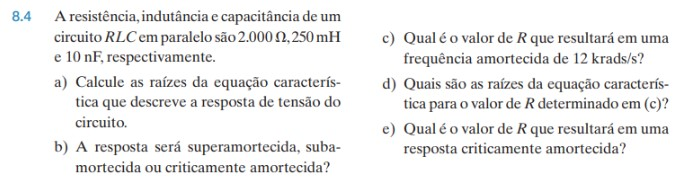
\includegraphics[scale=1.0]{P8.4.jpg}
\end{center}

\subsection*{(a)}

Sabemos que a equação característica da EDO de um circuito RLC paralelo é dada por   

\begin{equation}\label{eq:8.4.1}
    s^2 + \frac{s}{RC} + \frac{1}{LC} = 0
\end{equation}

Substituindo os dados do problema em \eqref{eq:8.4.1}, temos    

\[ s^2 + 5 \cdot 10^4 s + 4 \cdot 10^9 = 0 \]

Aplicando Bhaskara,  

\[ s = \frac{-(5 \cdot 10^4) \pm \sqrt{(5 \cdot 10^4)^2 - 4(1)(4 \cdot 10^8)}}{2(1)} \]

\[ \boxed{s_1 = -10000 \un{rad/s} \quad , \quad s_2 = -40000 \un{rad/s} }  \]

\subsection*{(b)}

A resposta da tensão depende do valor de $\Delta$ da equação característica, usada no item (a). Assim,   

\[ \Delta = (5 \cdot 10^4)^2 - 4(1)(4 \cdot 10^8) \]

\[ \Delta = 9 \cdot 10^{8} \]

Como $\Delta > 0$, temos que a resposta é superamortecida.

\subsection*{(c)}

A frequência angular amortecida $\omega_d$ é definida como  

\begin{equation}\label{eq:8.4.2}
    \omega_d = \sqrt{\omega_o^2 - \alpha^2}
\end{equation}

onde $\omega_o$ é a frequência angular de ressonância e $\alpha$ é o fator de armotecimento. Expandindo esses dois termos conforme suas definições, 
\eqref{eq:8.4.2} se torna  

\[ \omega_d = \sqrt{\left(\frac{1}{\sqrt{LC}}\right)^2 -  \left(\frac{1}{2RC}\right)^2} \]

\[ \omega_d = \sqrt{\frac{1}{LC} -  \frac{1}{4R^2C^2}} \]

Isolando $R$, temos   

\[ \omega_d^2 = \frac{1}{LC} -  \frac{1}{4R^2C^2} \]

\[ \frac{1}{R^2} = - 4C^2\left(\omega_d^2 - \frac{1}{LC}\right)\]

\[ R = \sqrt{\frac{1}{- 4C^2\left(\omega_d^2 - \frac{1}{LC}\right)}} \]

Substituindo $\omega_d = 12 \un{krad/s}$ e os demais valores do enunciado, temos  

\[ \boxed{R = 3125 \un{$\Omega$} }  \]

\subsection*{(d)}

Com $R = 3125 \un{$\Omega$}$ em \eqref{eq:8.4.1}, 

\[ s = \frac{-(3.2 \cdot 10^4) \pm \sqrt{(3.2 \cdot 10^4)^2 - 4(1)(4 \cdot 10^8)}}{2(1)} \]

\[ s = \frac{-(3.2 \cdot 10^4) \pm \sqrt{-5.76 \cdot 10^8}}{2(1)} \]

Note que agora temos que usar raízes complexas pois $\Delta < 0$.

\[ s = \frac{-(3.2 \cdot 10^4) \pm j(2.4 \cdot 10^4)}{2(1)} \]

\[ \boxed{s_1 = - 16000 + j12000\un{rad/s} \quad , \quad s_2 = - 16000 - j24000 \un{rad/s} }  \]

\subsection*{(e)}

Para que o circuito seja criticamente amortecido, precisamos de $\Delta = 0$. Assim, novamente usando \eqref{eq:8.4.1},  

\[ \Delta = \left(\frac{1}{RC}\right)^2 - 4(1)\left(\frac{1}{LC}\right) = 0 \]

Isolando $R$,

\[ \frac{1}{R^2C^2} = 4\frac{1}{LC} \]

\[R = \sqrt{\frac{1}{4C^2\frac{1}{LC}}} \logo R = \frac{1}{2}\sqrt{\frac{L}{C}} \]

Substituindo os valores do enunciado,  

\[ \boxed{R = 2500 \un{$\Omega$} }  \]










